\documentclass{article}

\usepackage[margin=1in]{geometry}
\usepackage{amsmath,amssymb}
\usepackage{graphicx}

\renewcommand{\thesection}{\arabic{section}}

\begin{document}

\title{Project AI \\ Auto-Encoding Stochastic Gradient Variational Bayes}
\author{	
	Joost van Amersfoort \\ 10021248  
	\and
	Otto Fabius \\ 5619858
	}
\maketitle

\section{Introduction}

In Machine Learning, it is often useful to model data as being generated from some underlying process, or hidden variables, according to some parametrized model. A powerful way to determine these parameters and latent variables (commonly grouped together as "unobserved variables") is to perform Bayesian Inference in order to obtain the MAP estimate. The resulting integral is, however, intractable, and is in practice approximated by a family of techniques known as Variational Bayes. These techniques have various drawbacks such as limited scalability or limited performance. \\
%referenties!
Recently, Kingma and Welling \cite{kingma2013auto} submitted a paper to ICLR 2014, where they present a new Variational Bayesian method, of which experimental results show it to be a large improvement over existing methods. In this report, we describe the novelty that is introduced and investigate several applications. Specifically, we try to replicate the results of Kingma and Welling by implementing the auto-encoder that they describe in the paper. After this replication step, that confirms our implementation works as it should, we test if using the auto-encoder to transform our data improves classification. Furthermore, we test the hypothesis that performing classification on the features is more robust to overfitting. 

\section{AEVB}

\subsection*{Problem class}

The problem class associated with AEVB is that where data $\mathbf{X}$ is assumed to be produced by some underlying process involving (continuous) hidden variables $\mathbf{Z}$. We can express the posterior probability over $\mathbf{X}$ by reformulating Bayes' Rule:

\begin{align}
P(X) = \frac{P(X|Z)P(Z)}{P(Z|X)}
\end{align}

Where $P(X|Z)$ and $P(Z|X)$ are parameterized by $\theta$.
\\

Knowing the probability distributions $P(X|Z)$ and $P(Z|X)$, i.e. learning $\theta$, can sometimes provide information on some natural process (if one is interested in the values of the parameters, for example). But knowing the distribution $P(Z|X)$ also allows us to infer $\mathbf{Z}$ from $\mathbf{X}$ to reduce the dimensionality of (encode) our data and find structure in the data. Furthermore, introducing a prior $P(Z)$ allows for computing the marginal probability $P(X)$ to generate data for applications such as image inpainting, denoising and super-resolution.
We would like to learn $\theta$ by gradient ascent/descent by differentiating some objective w.r.t. $\theta$. This can be done by choosing the marginal likelihood $P(X) = \int \frac{P(Z)}{P(X|Z)}dZ$ as objective to maximize, or by using the EM algorithm on the posterior density $ P(Z|X) = \frac{P(X|Z)P(Z)}{P(X)}$. However, calculating either  the marginal likelihood or the posterior density becomes intractable as the likelihood function $P(X|Z)$	 becomes more complex, which severely limits these methods. (possible e.g. variational linear regression, Bishop p. 486)





%In the class of problems we are interested in, the following conditions apply:
%\begin{itemize}
%\item The posterior distribution $P(Z|X)$ is intractable. 
%\item the probability density functions of the prior $P(Z)$ and the likelihood $P(X|Z)$, respectively, are differentiable w.r.t. $\mathbf{Z}$ and $\theta$. 
%\end{itemize}

\subsection{Sampling to obtain gradients}

Introducing $q(Z|X)$, parameterized by $\phi$, as an approximation of the posterior $P(Z|X)$, \cite{kingma2013auto} derive an expression for the Monte Carlo estimate of the lower bound $\mathcal{L}$ of the marginal likelihood $P(X)$:

\begin{align}
\mathcal{L}(\theta ,\phi ,  \mathbf{x^{(i)}}) \backsimeq \frac{1}{L} \sum_{l=1}^{L} \text{log } p_{\theta} (x^{(i)}|z^{(l)})+ \text{log }p(z^{(l)}	)-\text{log }q_{\phi}(z^{(l)}|x^{(i)})
\end{align}

Here, $z$ is sampled $l$ times from $q_{\phi}(z|x)$ for each datapoint $x^{(i)}$. Because $z$ therefore depends on parameters $\theta$, differentiating $\mathcal{L}$ w.r.t. $\phi$ will lead to a gradient which is influenced by the current parameters $\phi$. 
As a solution to this problem, \cite{kingma2013auto} reparameterize the samples of $z$ from $q(z|x)$ as
\begin{align}
z = g_\phi(\mathbf{\epsilon},\mathbf{x}) \text{  with  } \mathbf{\epsilon} \sim p(\mathbf{\epsilon}) 
\end{align} 

Now, once we have a sample $\epsilon$, the MC-estimate of $\mathcal{L}$ (equation (1) ) does not depend on a \textit{sampled} $z$, but on a  $z$ which is \textit{calculated deterministically}, independent of $\phi$. Thus, $\mathcal(L)$ can now be differentiated w.r.t all the parameters $\theta$ and $\phi$, enabling parameter optimization by means of stochastic gradient ascent.

\subsection{Modelling the conditional distributions}
For our experiments, we approximate $P(X|Z)$ and $q(X|Z)$ as neural networks with a single hidden layer, similar to \cite{kingma2013auto}. These neural networks can be trained well with backpropagation of error derivatives. They are also powerful, in the sense that they are universal approximators, i.e. they can approximate any function of their input. 

\section{Auto-encoders}

In the paper, Kingma and Welling implement an auto-encoder based on the reparametrization trick. Auto-encoders, or autoassociators as \cite{bengio2009learning} calls them, are trained to encode the input in some representation so that the input can be reconstructed from that representation. In a simple network with one hidden layer that has a linear activation function and is trained with the mean squared error criterion, the hidden units learn the principal components of the data (PCA). However, if the hidden units have a non-linear activation function, the auto-encoder learns much more interesting things.

An important application of auto-encoders, as \cite{bengio2009learning} describe, is as building blocks for a deep multi-layer neural network. An example of this application is to first train an auto-encoder on unlabeled data, then another auto-encoder is trained on the output of the hidden units of the first auto-encoder. This step can be repeated as many times as necessary. The last step is to train a supervised neural network on the output of the stacked auto-encoder. The supervised criterion can then be used tune all the parameters of deep network. 

However, for many classes of probabilistic models there is no tractable estimator for the log-likelihood. Therefore, in practice Restricted Boltzmann Machines are used as building blocks and the network is called a Deep Belief Network, as described in detail in \cite{hinton2006reducing}.


\section{Experiments}

In this section, we outline our experiments and present our results. We will present and discuss our results immediately after the description of each experiment so it is clear to the reader which results and conclusion belong to which experiment.

\subsection{Reproducing results}

Firstly, we performed some experiments to reproduce the results of \cite{kingma2013auto}. This way, we can verify the correctness of our implementation. In their paper, an Auto-Encoder was trained on both binary valued data (MNIST handwritten digits) and continuous valued data (Frey Faces \footnote{Available at http://www.cs.nyu.edu/ ̃roweis/data.html}).

\subsubsection{MNIST}

We first trained an auto-encoder with 400 hidden units and 20-dimensional latent space with SGD-VB on MNIST, in order to compare the lower bound of the log likelihood with \cite{kingma2013auto}. Figure 1 shows the lower bound per data point during training for both the training set and the test set. Figure 2 shows a manifold of generated data from an auto-encoder trained two-dimensional latent space and 400 hidden units. To create this visualization it is first necessary to create a 2D grid of vectors of the latent variables, such that each vector represents an equal probability mass from $p(z)$. Each data point was then generated by calculating the mean outputs of the trained auto-encoder on the values of the grid. The position in the total image reflects the coordinates of the hidden space. \\ 

\begin{figure}[htb]
\begin{center}
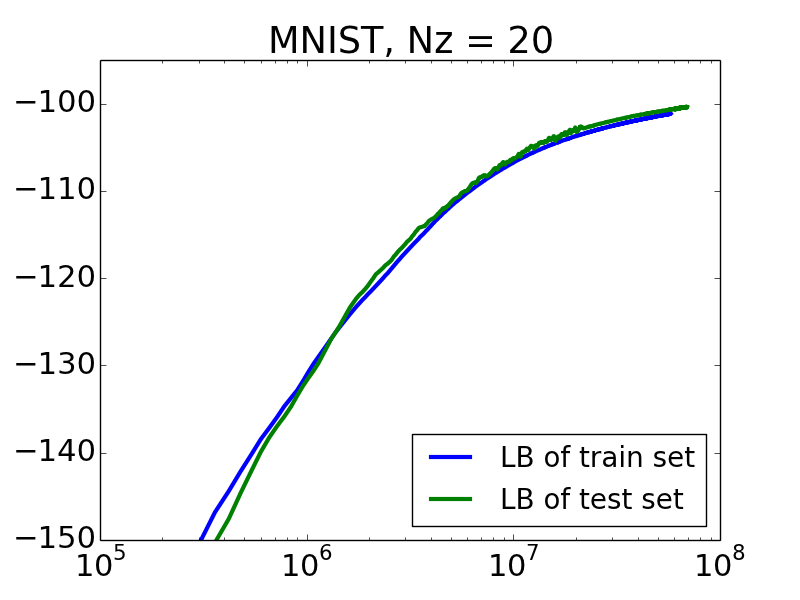
\includegraphics[height=3.1in,width=4in]{lowerboundAEVBMNIST.png}
\caption{Lower bound of the log likelihood per data point of both the train and test data during training}
\end{center}
\end{figure}

Also, we trained an auto-encoder with two-dimensional latent space in order to generate data for varying values of the latent variables along both latent dimensions. The resulting manifold is shown in Figure 2.

\begin{figure}[htb]
\begin{center}
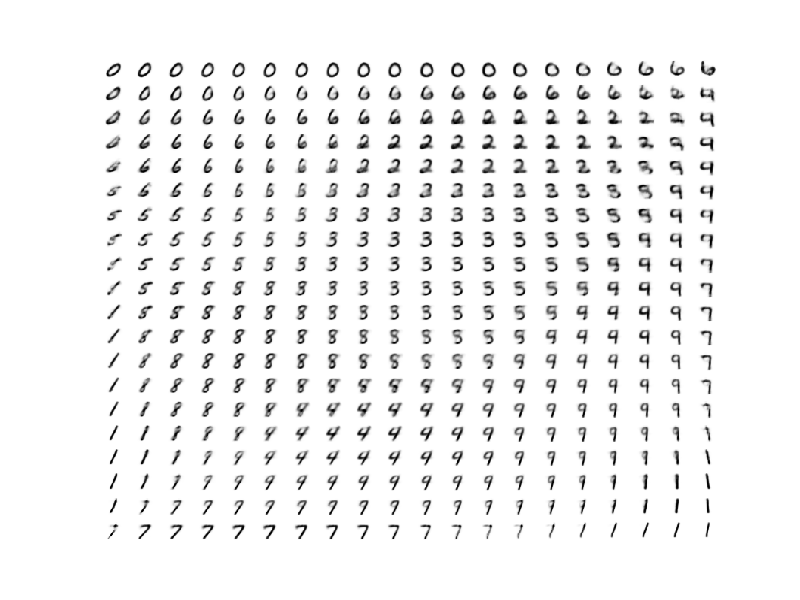
\includegraphics[height=4in,width=5in]{manifoldMNIST.png}
\caption{2D Manifold of MNIST}
\end{center}
\end{figure}

\subsubsection{Frey Faces}

Also for the continuous valued Frey Face dataset, we trained an auto-encoder with SGVB to compare the progression of the lower bound to that in \cite{kingma2013auto}. Figure 3 shows the lower bound of the training and test set as training progresses for latent dimensionality of 10, with 200 hidden units. Figure 4 shows a manifold of the Frey Face dataset, created in a similar fashion to what we describe in 4.1.1.

\begin{figure}[htb]
\centering
\begin{minipage}{0.5\textwidth}
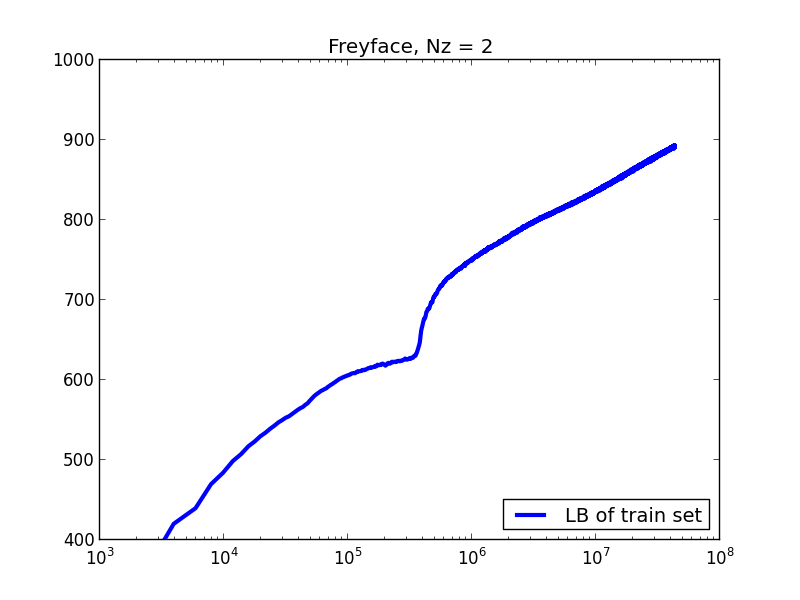
\includegraphics[height=3in,width=3.6in]{lowerboundFF.png}
\caption{Lower bound of the log likelihood per datapoint of the Frey Face dataset during training}
\end{minipage}%
\centering
\begin{minipage}{0.5\textwidth}
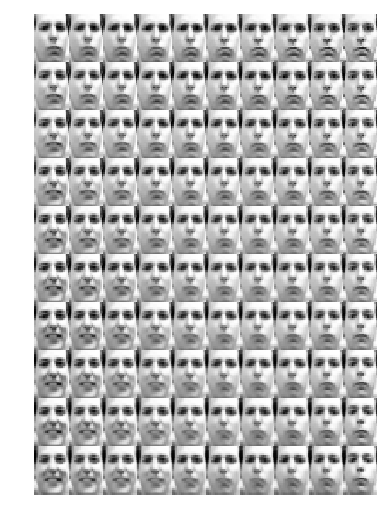
\includegraphics[height=3.2in,width=3.2in]{manifoldFF.png}\caption{2D Manifold of Frey Face}
\end{minipage}
\end{figure}

Training an auto-encoder with 200 hidden units and 2 latent dimensions once again enables visualization of generated data along both dimensions, shown in Figure 4.

These results achieved with our implementation of SGDVB auto-encoders are very similar to those to those presented in \cite{kingma2013auto}, which shows that our implementation is correct and that these results can be achieved consistently. 

\subsection{Classification}

In the remainder of the experiments, we will focus on one useful application of learned features, namely in classification. Before we use a classification method, we can use a trained Auto-Encoder to extract features from the data by calculating the output of the hidden layer of the Auto-Encoder. This way, we aim to improve the results of classification (supervised learning) with SGDVB (unsupervised learning). In particular, we will examine the performance of logistic regression on various representations of the same dataset. Classifying on features calculated by a one-layer neural network effectively results in a two-layered MLP, of which the first layer is not trained with supervised learning after training it with SGDVB. We compare obtained results to those obtained when using features trained with a Restricted Bolzmann Machine, which is a popular method for such (??) feature extraction and is frequently used for weight initialization in layers of deep belief nets (e.g. \cite{bengio2007greedy} ).

\subsubsection{Classifying MNIST on features}

In this subsection, we detail how well logistic regression performed on MNIST when using raw pixel data as input, features learned with an SGDVB Auto-Encoder as input, and with features learned with an RBM as input. \\ For this, we used the same Auto-Encoder of which the lower bound is shown in Figure 1. Thus, it has 400 hidden units and latent dimensionality of 20, was trained on approximately $5.0\cdot 10^7$ training examples, and reached a lower bound of $-101.53$ on the log likelihood per data point. The trained RBM also contained 400 hidden units to ensure the same representational power, and was trained on $1.5\cdot 10^7$ training examples from the MNIST training set. This yielded the same results as $0.5\cdot 10^7$ training examples and thus was enough iterations for convergence. This auto-encoder is used in several experiments later. \\
Logistic regression was run until results on the validation set declined or stabilized. The results are shown in Table 1.

\begin{table}
\begin{tabular}{|l|c|c|r|}
\hline
& Raw Data & SGVB AE Features & RBM Features \\ \hline
No. of training examples until convergence ($\cdot 10^6$) & 1.5 & 4.0 & 3.0 \\ \hline 
Test set accuracy & 93.36 & 97.54 & 96.29
\end{tabular}
\end{table}

As expected, using features calculated with the trained RBM improved the test set accuracy. However, the results using the trained auto-encoder were even better, leading to an error rate of only 2.46\%! This is an important finding, as auto-encoding SGVB proves to be a at least viable alternative to using an RBM for unsupervised learning. Besides outperforming RBMs (at least for this task), AE SGVB is theoretically more attractive than RBMs as it has a clearer objective that is maximized, and allows for calculating the lower bound, allowing for (efficient) monitoring during optimization and comparison  of lower bound across various parameter settings.\\
As the features were extracted from a one-layer neural network, this result was effectively achieved with a two-layer neural network, and it compares well to the 'classic' results achieved with two-layer NNs by \cite{lecun1998gradient}, who was only able to further improve results by deskewing. In this experiment, the first layer was not trained beyond unsupervised learning. Training both layers of the neural network during supervised learning could therefore further improve results.

\subsubsection{Classifying Chinese characters}

To investigate whether the boost in classification accuracy generalizes (at least in part) to other data, we also performed classification on the handwritten Chinese character dataset (voetnote, referentie of iets). \\
This dataset consists of 1,121,749 annotated datapoints in 3,750 different classes, with each class containing approximately the same number of characters. Each datapoint contains grey values of an image of a handwritten Chinese character and a code for its corresponding class. For preprocessing, we binarized the images and scaled them to 40x40. This is still larger than MNIST, which has dimensions 28 x 28 but was deemed necessary to keep the more fine grained structure of the characters intact. As images had varying aspect ratios, we added white padding whenever necessary, in order to have constant dimensionality of the data. Due to resource and time limitations, we only used 50 classes, resulting in 11,578 data points. The resulting dataset is similar to MNIST in size and type, but considerably more complex in that the images are larger, there are 5 times as many classes, and the structure in the images is more complex.\\
Once again, we trained an auto-encoder on the data, and used logistic regression to classify the data. For the auto-encoder, we used 500 hidden units and hidden dimensionality of 200. The auto-encoder is trained on the 10,000 images in the train set and the lower bound on the log likelihood during training is shown in Figure 5. 

\begin{figure}[htb]
\begin{center}
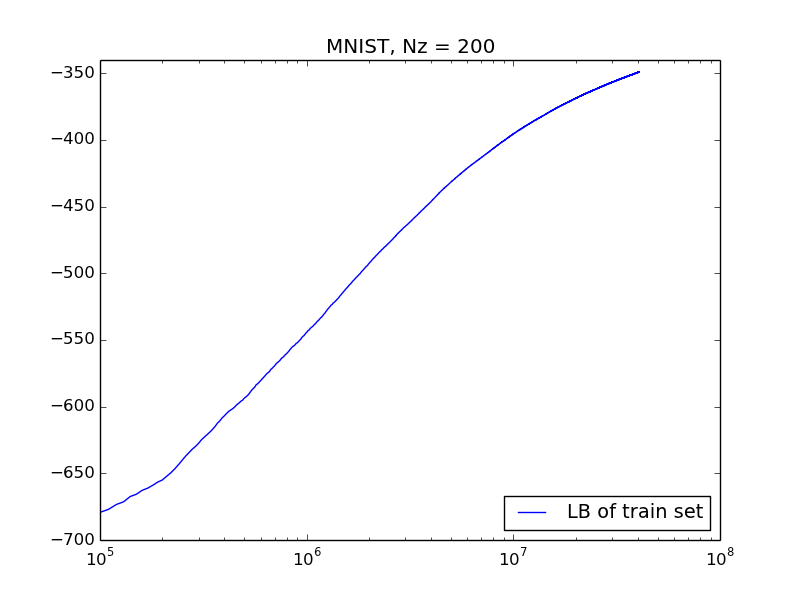
\includegraphics[height=3.1in,width=4in]{lowerboundchinese.png}
\caption{Lower bound of the log likelihood per datapoint of the train set during training.}
\end{center}
\end{figure}

Once again, we trained a classifier with logistic regression on both the preprocessed pixel values as well as the features extracted from the trained encoder. \\
Logistic regression on the pixel values yielded a test set accuracy of 66.29\%, compared to 69.17\% when classifying on the features. Percentage-wise, this is a similar increase in accuracy as achieved on MNIST, but as the scores are much lower than on MNIST, this increase is relatively small. \\
It is not obvious whether this indicates whether the learned features are less effective for this dataset than for MNIST. If so, one possible explanation is that the lower bound had not converged as much as the lower bound for MNIST (see Figure 1). Additional experiments, such as training the auto-encoder longer, training an RBM to extract features to classify on, and training on a larger part of the Chinese character dataset could provide more insight in the effectiveness on SGVB auto-encoders for use in classification in general and for the Chinese character dataset in particular.


\subsubsection{Classification on Small Datasets}

In practice it is hard to obtain large annotated datasets for supervised learning. Therefore, we also tested the effectiveness of learned features for improving the classification results for small subsets of MNIST. Once again, logistic regression is our classification method of choice. In addition to features calculated with the auto-encoder trained earlier (see Figure 1), a two-layer auto-encoder was trained with SGVB. This was done by stacking another auto-encoder on top of the first auto-encoder. This was done simply by using the features, computed by the first auto-encoder, as input for SGD to train a new auto-encoder as before. Since the values of these computed features are continuous, as opposed to the pixel data, the second auto-encoder was trained to approximate Gaussian distribution instead of a Bernoulli distribution, as discussed earlier. For the second auto-encoder, once again 400 hidden units and latent dimensionality of 20 were chosen to be able to compare the results. The resulting features for the two-layer autoencoder are then computed through the following formula. Note that the output of the first hidden layer is normalized between 0 and 1.

\begin{align}
    f = \log(1 + \exp[-(\tanh(\textbf{W}^T*\textbf{X} + \textbf{b}) + 1)/2])
\end{align}

In our experiment, we selected the first $x$ training examples from the training set of MNIST as our training set, where $x$ started at 4 and was increased each time by multiplying it with 2, up to a size of 2048. To evaluate the results for each dataset size, we used the first 1000 data points of the MNIST test set and validation set, respectively.\\
Figure 6 shows the accuracy on the test set after training logistic regression on the first $x$ data points of MNIST until accuracy on the validation set converged. The results show that training on the features computed with the one-layer auto-encoder yield better results across the whole range of used dataset sizes, in addition to using the full dataset (see 3.2.1). The two-layer auto-encoder shows an additional boost in performance for dataset sizes of up to 64 total datapoints, but is less effective for larger datasets. \\

\begin{figure}[htb]
\begin{center}
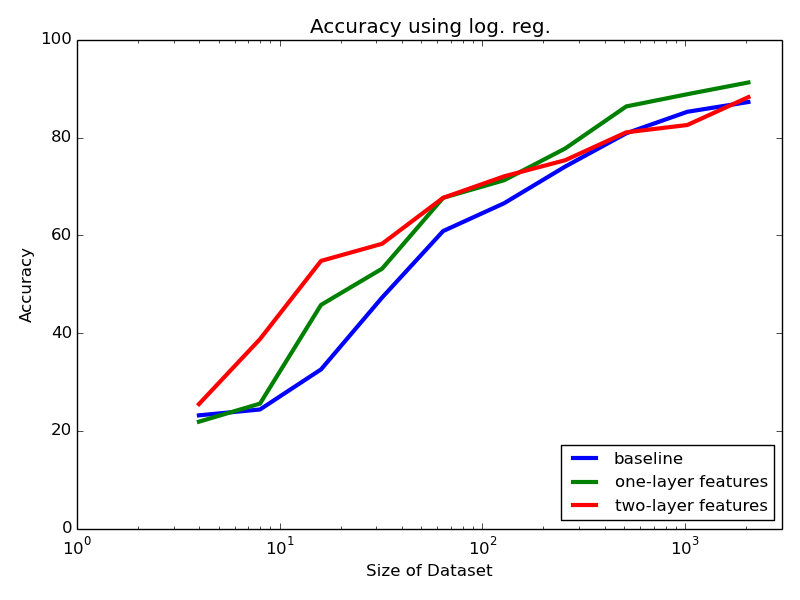
\includegraphics[height=4in,width=5in]{logreg_smallsets_report.png}
\caption{Lower bound of the log likelihood per datapoint of the train set during training.}
\end{center}
\end{figure}

These results show that also for small datasets, unsupervised learning with SGVB auto-encoders can increase the effectiveness of classification algorithms. As in logistic regression on the full dataset, the resulting two- and three-layer MLPs were not trained as a whole on supervised data. Also, the layers of the two-layer auto-encoder were trained independently, while jointly training all the parameters could fine tune the parameters to obtain better features. These possibilities can be explored further in future experiments. Also, training and effectively fine-tuning multilayer auto-encoders with SGVB seems very promising from these somewhat preliminary results. 

\subsection{Generalizability of Features}

One of the advantages of extracting a set of relevant features of data, in general, is that performing classification on these features is more robust to overfitting than performing classifications on the original data.  In this subsection, we detail an experiment designed to test the extent to whether this general property of features is applicable to the feature representation generated with the trained auto-encoder described earlier.\\
We chose a Support Vector Machine with a Radial Basis Function kernel as our classification method, since the susceptibility of this method to overfitting is easily manipulable by setting the precision of the RBF kernel. Too high values for this hyperparameter will lead to overfitting, while too low values will prevent overfitting, but at the cost of reducing the discriminative power (and thus, accuracy). As the robustness to overfitting is particularly desirable when training on a small dataset, we trained a Support Vector Machine on small subsets of the training set of MNIST, as well as on the features extracted from the same data using the trained auto-encoder. Once again, we used the first 1000 examples from the MNIST test set to calculate the test accuracy.\\
The achieved train and test set accuracy across different dataset sizes are shown for different settings of the precision of the RBF kernel in Figure 7. It is clearly visible that for larger precision, classifying on pixel values is heavily outperformed by using the kearned features. Using the features yields acceptable results even whith $\gamma = 0.3$, where this leads to such severe overfitting on the pixel values that the resulting classifier barely performs better than random on the test set.\\
These results clearly demonstrate the robustness to overfitting that comes from learning a feature representation of data. This further improves the utility of SGVB as a method to improve classification algorithms, especially when annotated data is scarce. Presumably, these results are compounded when higher-level features are extracted from the data. Once higher-level features have been extracted effectively with SGVB, this experiment can be repeated to investigate this further.




\begin{figure}[htb]
\centering
\begin{minipage}{0.36\textwidth}
\includegraphics[height=2in,width=2.5in]{svm001.png}
\end{minipage}%
\centering
\begin{minipage}{0.36\textwidth}
\includegraphics[height=2in,width=2.5in]{svm003.png}
\end{minipage}\\
\centering
\begin{minipage}{0.36\textwidth}
\includegraphics[height=2in,width=2.5in]{svm01.png}
\end{minipage}%
\centering
\begin{minipage}{0.36\textwidth}
\includegraphics[height=2in,width=2.5in]{svm03.png}
\end{minipage}
\caption{Results of classification on MNIST with a SVM with RBF kernel. Precision of the RBF kernel (Gamma) is set to different values, as denoted above each plot.}
\end{figure}

\subsection{Regularization effect of the lower bound}
Kingma and Welling \cite{kingma2013auto} claim that the lower bound has a regularizing effect on the usage of dimensions of Z. This would be a welcome property as it would not be necessary to tune this hyper-parameter. Furthermore, by inspecting the L2 norm of the weights during training it is possible to figure out which dimensions are not being `used'. With this information it becomes possible to prune these dimensions and save computations and time in future iterations.

We performed an experiment in which we trained an auto-encoder with a dimensionality of Z of 20 and 400, and 400 hidden units on MNIST. The results can be seen in the following figures:

\begin{figure}[htb]
    \centering
    \begin{minipage}{0.36\textwidth}
        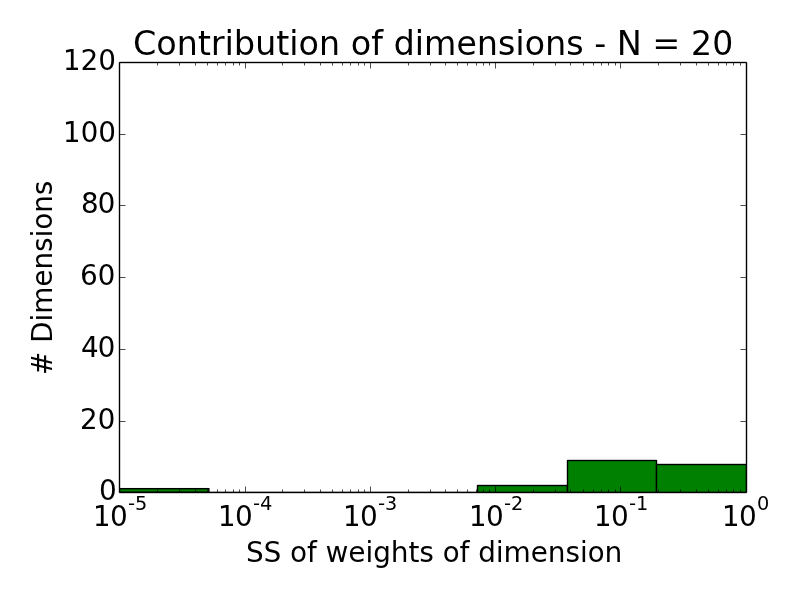
\includegraphics[height=2in,width=2.5in]{relevant_z_N20.png}
    \end{minipage}
    \centering
    \begin{minipage}{0.36\textwidth}
        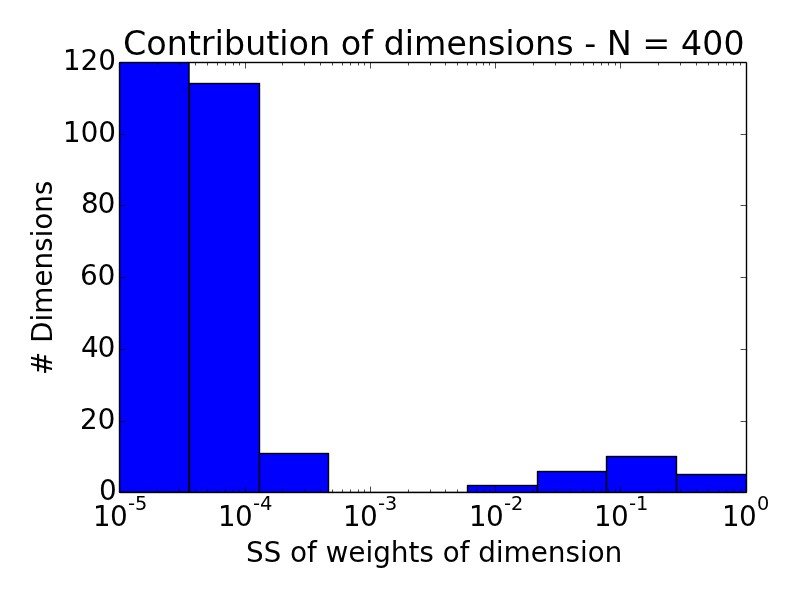
\includegraphics[height=2in,width=2.5in]{relevant_z_N400.png}
    \end{minipage}
    \caption{Sum of squares of the dimensions of W4 (weights for decoder)}
\end{figure}

In these two figures it can clearly be seen that around 20 dimensions is sufficient to encode the necessary information. Adding more dimensions will not substantially change the result as the weights of those dimensions are negligible.


\section*{Conclusion}

In our experiments, we found that the results as described by \cite{kingma2013auto} are indeed reproducible by implementing the theory as laid out in the paper. We also conclude that performing classification on the features learned by the auto-encoder gives a higher score for MNIST as well as Chinese characters. Notably, the boost in performance is higher than what was achievable with RBMs. Another conclusion we can draw from our results is that training on features of the auto-encoder is more robust to overfitting. 

For further research, there are several interesting opportunities. First, we have already shown that it is possible to beat the current state-of-the-art on simple classifications problems with simple classification methods. It would be interesting to find out how the variational auto-encoder performs on more complicated problems and with more complicated classification methods. Second, several common applications of auto-encoders, such as denoising and superpixeling, are not tested yet. Last, the auto-encoder could be used as a building block in a deep neural network, replacing RBMs. Given the theoretical advantages of the variational auto-encoder and the shown improved results, it is possible that this will perform better than the current state-of-the-art.


\pagebreak 
\bibliographystyle{amsplain}
\bibliography{references.bib}

\end{document}
